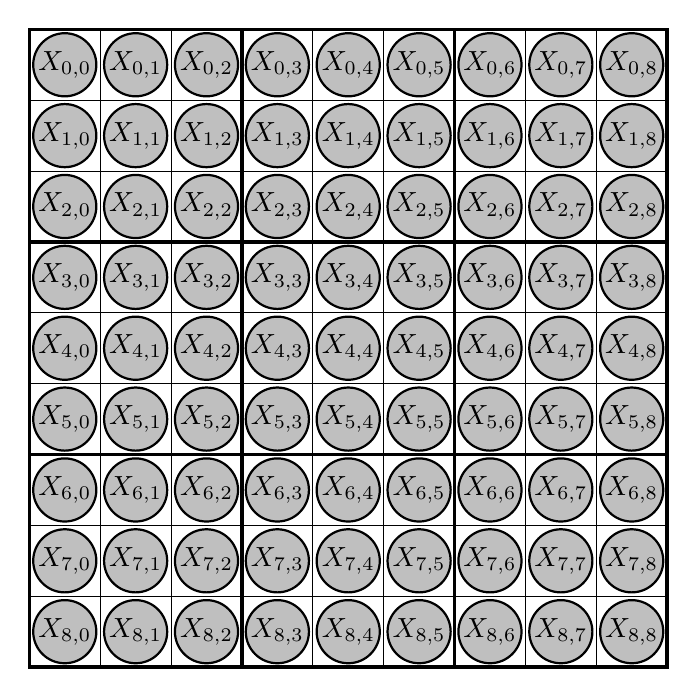
\begin{tikzpicture}[scale=0.9]
% Draw the main grid

%\node[anchor=center] (text) at (0,9) {${a)}$};

\draw[very thick] (0,0) rectangle (9,9); % Outer border
\foreach \x in {1,2,...,8} {
    \draw[thin] (\x,0) -- (\x,9); % Vertical lines
    \draw[thin] (0,\x) -- (9,\x); % Horizontal lines
}
% Thicker lines for 3x3 subgrids
\foreach \x in {3,6} {
    \draw[very thick] (\x,0) -- (\x,9); % Vertical thick lines
    \draw[very thick] (0,\x) -- (9,\x); % Horizontal thick lines
}

% Add variables in the middle of each square
\foreach \i in {0,1,...,8} {
    \foreach \j in {0,1,...,8} {
        \node[circle, draw, thick, fill=gray!50, inner sep = 0.5pt, minimum size=0.6cm, align=center] 
        at (\j+0.5,8-\i+0.5) {$X_{\i,\j}$};
    }
}

%\begin{scope}[shift={(2,0)}]
%
%\node[anchor=center] (text) at (9,9) {${b)}$};
%	
%% Draw a line of variables (horizontal)
%\foreach \k in {0,1,...,8} {
%    \node[circle, draw, thick,  fill=gray!50, inner sep=0pt, 
%    minimum size=0.6cm, align=center] 
%    at (10+\k,8.5) {$X_{i,\k}$};
%}
%
%\node[anchor=center] (text) at (9,7) {${c)}$};
%
%% Draw a column of variables (vertical)
%\foreach \l in {0,1,...,8} {
%    \node[circle, draw, thick, fill=gray!50, inner sep=0pt, 
%    minimum size=0.6cm, align=center] 
%    at (10,-\l+6) {$X_{\l,j}$};
%}
%
%\node[anchor=center] (text) at (9,7) {${d)}$};
%
%% Draw a square of variables (3x3)
%\foreach \i in {0,1,2} {
%    \foreach \j in {0,1,2} {
%        \node[circle, draw, thick, fill=gray!50, inner sep=0pt, 
%        minimum size=0.6cm, align=center] 
%        at (12+\j,6-\i) {$X_{\i,\j}$};
%    }
%}
%
%\end{scope}

\end{tikzpicture}
